\documentclass{school-22.211-notes}
\date{March 14, 2012}

\begin{document}
\maketitle

\lecture{Intro to Diffusion Theory}
\topic{Why We Need Deterministic Codes}
Monte Carlo produces accurate results (as demonstrated by our very simplified tool), but it requires too much computer power:
\begin{itemize}
\item Using our tool as an example, it takes about 14,000 CPU for one calculation of a full core (70,000 pins, 50 pcm). 
\item BETTIS/KAPL's MC21: one state-point, no feedback, 1 billion tallies, about 200 billion active neutron histories, for 1\% 95/95 pin-power uncertainty, we are looking at 100 hours on 1000 ciores. 
\end{itemize}

Hence we turn to deterministic codes, like diffusion theory. Common neutronics applications includes: 
\begin{enumerate}
\item 2D Lattice transport/depletion calculation: approximate boundary conditions;
\item 3D simulation using few group diffusion models: 
  \begin{enumerate}
  \item 3D Pin Approach: solve unique pins or lattice in detail; treat each pin as homogenized; solve 3D homogenized pin few-group diffusion problem. 

  \item 3D Noval Approach: solve unique lattice in detail; treat each assembly as homogenized; solve 3D homogenized-asssembly few-group diffusion problem. 
  \end{enumerate}
  The only difference between 3D pin approach and 3D noval approach is to treat a pin as a node vs. to treat an assembly as a node. For BWRs, that's about 2-3\% difference in power; for PWRs, that's only 1\% difference in power. 
\end{enumerate}


\clearpage
\topic{k-infinity Formalism}
The general definition of $\kinf$ is\footnote{Reference: Henry p. 104, Lec10},
\eqn{ \kinf =  \frac{\mbox{total fissions} \cdot \bar{\nu} }{\mbox{total absorptions}} = \frac{\int \dV \int \nu \overline{\Sigma_f} \Phi \dE}{\int \dV \int \overline{\Sigma_a} \Phi \dE} = \epsilon \eta f p }

\begin{enumerate}
\item $k$ from One-Group Cross Section. We start by writing down the One-Group Balance Equation, 
\eqn{ \frac{\nu \bar{\Sigma}_f}{\kinf} \phi - \bar{\Sigma}_a \phi = 0}
Rearranging, we get 
\eqn{ \kinf = \frac{\nu \bar{\Sigma}_f \phi}{\bar{\Sigma}_a \phi} = \frac{\nu \bar{\Sigma}_f }{\bar{\Sigma}_a} }
Observations:
\begin{itemize}
\item $\kinf$ is simply the ratio of total neutron production to destruction rate;
\item $\kinf$ does not depend on flux magnitude, normalization, etc;
\item $\kinf$ depends only on integrated cross sections;
\item Cross sections for down stream codes which treat pin-cells as homogenized will preserve exactly our MC fuel reactivity for infinite repeating lattices. 
\item Notice $\kinf$ assumes no leakage; $\keff$ would add an leakage term,
  \eqn{ \keff = \frac{\nu \Sigma_f}{DB^2 + \Sigma_a} }
\end{itemize}


\item $k$ from Two-Group Cross Section. Again we start with the neutron balance equations (assume all neutrons born in fast group):
\eqn{\frac{\nu \bar{\Sigma}_{f1}}{\kinf} \phi_1 - \bar{\Sigma}_{a1} \phi_1 - \bar{\Sigma}_{s12} \phi_1 + \frac{\nu \bar{\Sigma}_{f2}}{\kinf} \phi_2 + \bar{\Sigma}_{s21} \phi_2 = 0} 
\eqn{\bar{\Sigma}_{s12} \phi_1 - \bar{\Sigma}_{s21} \phi_2 - \bar{\Sigma}_{a2} \phi_2 = 0 }
\begin{enumerate}
\item General case: we express the above expression in matrix form, 
  \begin{align}
    \left[ \begin{array}{cc} 
        \frac{\nu \bar{\Sigma}_{f1}}{\kinf} -  \bar{\Sigma}_{a1}  - \bar{\Sigma}_{s12} & \frac{\nu \bar{\Sigma}_{f2}}{\kinf}  + \bar{\Sigma}_{s21}  \\
        \bar{\Sigma}_{s12} & - \bar{\Sigma}_{s21} - \bar{\Sigma}_{a2}  
      \end{array} \right] 
    \left[ \begin{array}{c} \phi_1 \\ \phi_2 \end{array} \right] = 0
  \end{align}
  We set determinant to be zero and solve for $\kinf$. 

\item We define \hi{effective down-scattering cross section}, 
  \eqn{ \hat{\Sigma}_{s12} = \bar{\Sigma}_{s12} - \bar{\Sigma}_{s21} \frac{\phi_2}{\phi_1} }
  we define \hi{effective removal cross section} as,
  \eqn{ \Sigma_{rg} = \Sigma_{tg} - \Sigma_{sgg} = \Sigma_{ag} + \Sum_{g'=1, g'\neq g}^G \Sigma_{sgg'}  }
  Then the matrix form becomes, 
  \begin{align}
    \left[ \begin{array}{cc} 
        \frac{\nu \bar{\Sigma}_{f1}}{\kinf} -  \bar{\Sigma}_{a1}  - \hat{\Sigma}_{s12} & \frac{\nu \bar{\Sigma}_{f2}}{\kinf}   \\
        \hat{\Sigma}_{s12} &  - \bar{\Sigma}_{a2}  
      \end{array} \right] 
    \left[ \begin{array}{c} \phi_1 \\ \phi_2 \end{array} \right] = 0
  \end{align}
  The second row implies that, 
  \eqn{ \frac{\phi_2}{\phi_1} = \frac{\hat{\Sigma}_{s12} }{\bar{\Sigma}_{a2}} }
  Plug into the first row, we get, 
  \eqn{ \frac{\nu \bar{\Sigma}_{f1}}{\kinf} -  \bar{\Sigma}_{a1}  - \hat{\Sigma}_{s12} + \frac{\nu \bar{\Sigma}_{f2}}{\kinf}  \frac{\hat{\Sigma}_{s12} }{\bar{\Sigma}_{a2}} = 0 }
  \eqn{ \boxed{\kinf = \frac{\nu \bar{\Sigma}_{f1} + \nu \bar{\Sigma}_{f2} \frac{\hat{\Sigma}_{s12} }{\bar{\Sigma}_{a2}}}{\bar{\Sigma}_{a1} + \hat{\Sigma}_{s12} }   } }
  
  Notice that,
  \begin{itemize}
  \item Know how to derive the above expression;
  \item Two-Group $\kinf$ depends only on the intergrated cross sections;
  \item Although it looks like a chicken-to-egg problem that we include $\frac{\phi_2}{\phi_1}$ in $\hat{\Sigma}_{s12}$, my understanding is that we either know flux and needs to find cross section, or the other way around, hence we do not need to worry about this term. 
  \item If no upscattering, $\hat{\Sigma}_{s12}$ is effectively $\overline{\Sigma}_{s12}$.
  \end{itemize} 
\end{enumerate}

\item $k$ from Balance Equation. For two region problem, we can also solve $\kinf$ from the neutron balance equation. We can reduce down scattering cross section from balance equation (instead of from group-to-froup tallies), 
    \eqn{ \hat{\Sigma}_{s12} = \frac{\frac{\nu \bar{\Sigma}_{f1}}{\kinf} - \bar{\Sigma}_{a1} }{1 - \frac{\nu \bar{\Sigma}_{f2} }{\kinf \bar{\Sigma}_{a2}}}}
\end{enumerate}

\textit{The $\kinf$ from the three methods above should agree, because reaction rates conserves}.


\clearpage
\topic{Derivation Of Diffusion Theory From Transport Theory}
\begin{enumerate}
\item Start from the steady state continuous energy transport equation: 
\eqn{ \vecOmega \cdot \gradient \psi(\vecr, E, \vecOmega) + \Sigma_t (\vecr, E) \psi(\vecr, E, \vecOmega) = \int \dE' \int \dOmega' \Sigma_s(\vecr, E'\to E, \vecOmega' \to \vecOmega) \psi(\vecr, E', \vecOmega') + S(\vecr, E, \vecOmega) }  

\item Expand scattering source/flux in spherical harmonics, integrate over angle $\dOmega$,
\begin{align}
 &\overbrace{\int_{4\pi} \dOmega \vecOmega \cdot \gradient \psi(\vecr, E, \vecOmega)}^{\textcircled{1}} 
+ \Sigma_t (\vecr, E) \overbrace{\int_{4\pi} \dOmega \psi(\vecr, E, \vecOmega)}^{\textcircled{2}} \\
&= \Sum_i \Sum_{l=0}^L \Sum_{k=-l}^l \overbrace{\left[\int_{4\pi} \dOmega Y_{lk} (\vecOmega) \right]}^{\textcircled{3}} \int \dE' \Sigma_s(\vecr, E'\to E) \psi_{lk}(\vecr, E') + \overbrace{\int_{4\pi} \dOmega S(\vecr, E, \vecOmega)}^{\textcircled{4}} 
\end{align}
The scattering kernel is nasty, because a) $\Sigma_s$ depends on energy, hence we have to integrate over all energy; b) $\Sigma_s$ depends on angle, hence we have to integrate over all angle; c) $\Sigma_s$ depends on isotope, hence we have to integrate over all isotopes. 

\item Simplify the four angle integrals,
\begin{align}
\textcircled{1} &= \int_{4\pi} \dOmega (\divergence \vecOmega \psi) = \divergence \left[\int_{4\pi} \dOmega \vecOmega \psi \right] = \divergence \vec{J} (\vecr, E) \\
\textcircled{2} &= \phi(\vecr, E) \\
\textcircled{3} &= \sqrt{4\pi} \int_{4\pi} \dOmega \bar{Y}_{00}(\vecOmega) Y_{lk} (\vecOmega) = \sqrt{4\pi} \delta_{l0}\delta_{k0}, \fsp \fsp \sqrt{4 \pi } \psi_{00} = \phi \\
\textcircled{4} &= S_0 (\vecr, E) 
\end{align}

\item We obtain the balance equation:
\eqn{ \boxed{ \divergence \vecJ (\vecr, E) + \Sigma_t (\vecr, E) \phi(\vecr, E) = \Sum_i \int_{E'} \dE' \Sigma_{s}^i (\vecr, E'\to E) \phi(\vecr, E') + S_0 (\vecr, E) }}
This balance equation is basically equalling the source and the sink. Notice this equation is exact so far. But since we do not know what $\vec{J}$ is, we need to approximate it somehow. 
\end{enumerate}

Basically going from transport to diffusion theory we drop the $\Omega$ dependency. Thus we define the scalar flux $\phi(\vecr, E)$ and the net current $\vecJ (\vecr, E)$: 
\eqn{ \int_{4\pi} \dOmega \psi(\vecr, E, \vecOmega) &= \phi (\vecr, E) & \int_{4\pi} \dOmega \vecOmega \psi(\vecr, E, \vecOmega) = \vecJ (\vecr, E) }

The only reason we brought up the transport theory is that we need to set the boundary condition right.  




\clearpage
\topic{Net Current Equation}
\begin{enumerate}
\item We start from transport equation again, multiple by $\Omega$ and integrate over all angles: 
\begin{align}
& \overbrace{\int_{4\pi} \dOmega \vecOmega \vecOmega \cdot \gradient \psi(\vecr, E, \vecOmega)}^{\textcircled{5}} 
+ \Sigma_t (\vecr, E) \overbrace{\int_{4\pi} \dOmega \vecOmega \psi(\vecr, E, \vecOmega)}^{\textcircled{6}} \\
&= \Sum_i \Sum_{l=0}^L \Sum_{k=-l}^l \overbrace{\left[\int_{4\pi} \dOmega \vecOmega Y_{lk} (\vecOmega) \right]}^{\textcircled{7}} \int \dE' \Sigma_{s1}^i (\vecr, E'\to E) \psi_{lk}(\vecr, E') 
+ \overbrace{\int_{4\pi} \dOmega \vecOmega S(\vecr, E, \vecOmega)}^{\textcircled{8}} 
\end{align}

\item Substitute the $P_1$ angular flux expansion, 
\eqn{ \psi(\vecr, E, \vecOmega) = \frac{1}{4\pi} \left[ \phi(\vecr, E) + 3 \vecOmega \cdot \vecJ(\vecr, E) \right] }
and recall four identities,
\begin{align}
\int_{4\pi} \dOmega &= 4 \pi, & \int_{4\pi} \dOmega \vecOmega &= 0 \\
\int_{4\pi} \dOmega \vecOmega \vecOmega \cdot \vec{A} &= \frac{4\pi}{3} \vec{A}, & \int_{4\pi} \dOmega \vecOmega \vecOmega \vecOmega &= 0 
\end{align}
We can simplify the angular integral terms:
\begin{align}
\textcircled{5} &= \frac{1}{4\pi} \int_{4\pi} \dOmega \vecOmega \vecOmega \cdot \gradient \phi + \frac{3}{4\pi} \int_{4\pi} \dOmega \vecOmega \vecOmega \cdot \gradient (\vecOmega \cdot \vecJ) = \frac{1}{3} \gradient \phi \\
\textcircled{6} &= \vecJ (\vecr, E) \\
\textcircled{7} \psi_{lk} &= \vecJ \\
\textcircled{8} &= \vec{S}_1 (\vecr, E) 
\end{align}

\item We obtain the net current equation:
\eqn{\boxed{ \frac{1}{3} \gradient \phi(\vecr, E) + \Sigma_t (\vecr, E) \vecJ(\vecr, E) = \Sum_i \int_{E'} \dE' \Sigma_{s1}^i (\vecr, E'\to E) \vecJ(\vecr, E') + \vec{S}_1(\vecr, E) } }
\end{enumerate}


\clearpage
\topic{Scattering and Diffusion Coefficients}
Start from the net current equation, assume the source is isotropic, then the source term goes away:
\eqn{ \frac{1}{3} \gradient \phi(\vecr, E) + \Sigma_t (\vecr, E) \vecJ(\vecr, E) = \Sum_i \int_{E'} \dE' \Sigma_{s1}^i (\vecr, E'\to E) \vecJ(\vecr, E')  }

Next we can either assume scattering to be isotropic in the Lab system, or isotropic in the Center of Mass system. 
\begin{enumerate}
\item Assume the scattering is isotropic in the Lab system, then the scattering kernel goes away:
\eqn{ \frac{1}{3} \gradient \phi(\vecr, E) + \Sigma_t (\vecr, E) \vecJ(\vecr, E) = 0} 
That is, 
\eqn{ \Aboxed{ \vecJ(\vecr, E) &= -D(\vecr, E) \gradient \phi(\vecr, E)} 
& D(\vecr, E) &= \frac{1}{3 \Sigma_t (\vecr, E)} }
This is the first way to calculate diffusion coefficient, that is, $D = \frac{1}{3 \Sigma_t}$. Notice the assumption of isotropic scattering in Lab system is not very good in a typical PWR -- because hydrogen scattering dominates, and hydrogen scatters isotropically in the COM system, not in the lab system. 


\item Assume the scattering is isotropic in the Center of Mass system. We use the \hi{transport correction $P_0$ approximation}:
\begin{align}
  \Aboxed{ D(\vecr, E) &= \frac{1}{3 \Sigma_{tr} (\vecr, E) } } \\
  \Aboxed{ \Sigma_{tr} (\vecr, E) &= \Sigma_t(\vecr, E) - \Sigma_{s1} (\vecr, E) } 
\end{align} 
\end{enumerate}


The transport cross section in the transport-corrected $P_o$ approximation for isotope $i$ is, 
\begin{align}
\sigma_{s1}^i (E\to E') &= 2 \pi \int_{-1}^1 \dmu_s \sigma_s^i (E\to E', \mu_s) P_1 (\mu_s) \\
&= \int_{-1}^1 \dmu_s \sigma_s^i (E \to E') \delta(\mu_s - \mu_s(E,E')) \mu_s \\
&= \mu_s (E', E) \sigma_s^i (E \to E') \\
\sigma_{s1}^i (E) &= \int_{E'} \dE' \mu_s(E,E') \sigma_s^i (E\to E') \\
&= \bar{\mu}^i (E) \sigma_s^i (E) \\
\sigma_{tr}^i (E) &= \sigma_t^i (E)  - \sigma_{s1}^i (E)  \\
&= \sigma_t^i (E) - \bar{\mu}^i (E) \sigma_s^i (E)
\end{align}
Under the assumption of isotropic scattering in COM, the mean value of cosine theta over the interval $-1,1$ is zero; the mean value of the cosine psi over the intervale $-1,1$ is $\frac{2}{3A}$, hence,
\eqn{ \boxed{ \sigma_{tr}^i (E) = \sigma_t^i (E) - \frac{2}{3 A^i} \sigma_s^i(E) } }
In summary, there are three ways to calculate diffusion coefficients: 
\begin{enumerate}
\item Assuming isotropic scattering in lab system, we can calculate the flux-weighted total cross section,
\eqn{ D &= \frac{1}{3 \Sigma_t},  &\Sigma_t &= \frac{\Sum \Sigma_t \phi}{\Sum \phi} }
\item Flux-weighted transport cross section: 
\eqn{ D &= \frac{1}{3 \Sigma_{tr}},& \Sigma_{tr} &= \frac{\Sum \Sigma_{tr} \phi}{\Sum \phi} }
The problem with this method is that flux collapse under-predict transport. 
\item Flux-weighted diffusion coefficient, and this is the most accurate one,
\eqn{ D &= \frac{\Sum \frac{1}{3 \Sigma_{tr}} \phi }{\Sum \phi} }


\end{enumerate}


\clearpage
\topic{Boundary Conditions}
Again, recall that the only reason we brought up transport theory in this course is to set the boundary condition straight. 
\begin{enumerate}
\item Zero flux boundary condition:
  \eqn{ \phi (0) = 0 }

\item Zero incoming flux boundary condition (more accurate than zero flux, because there could still be flux leaking out the geometry):
\eqn{ \left. \psi(\vecr, E, \vecOmega) \right|_{\vecn \cdot \vecOmega < 0} = 0}
Integrating over all angles in half space, that is incoming partial current is zero, 
\eqn{ J^- (\vecr_i, E) = 0}
There are two formulism to solve this:
  \begin{itemize}
  \item Kord's formulism: 
    \eqn{ J^- (\vecr, E) &= \frac{1}{4} \phi(\vecr, E) - \frac{1}{2} J_n (\vecr, E)  = 0, & \Aboxed{ \frac{J}{\phi} &= \frac{1}{2} } }
  \item The more conventional approach is to approximate with extropolation boundary condition: 
    \begin{align}
      J^- &= \frac{1}{4} \phi + \frac{D}{2} \gradient \phi_n \\
      \Aboxed{ \frac{\gradient \phi}{\phi} &= - \frac{1}{2D} = - \frac{3\Sigma_{tr}}{2} = - \frac{1}{d_{\mathrm{extrap}}}} 
\mbox{   where } d_{\mathrm{extrap}} = \frac{2}{3 \Sigma_{tr}}  = \frac{2}{3} \lambda_{\mathrm{tr}}
    \end{align}
    where $D$ is the property of the material inside, and $\lambda_{tr}$ is transport mean free path. Notice that the exact coefficient in $d_{\mathrm{extrap}}$ may be different. Take into account that thermal neutron mean free path is on the order of 1cm, so $d_{\mathrm{extrap}}$ is even less than 1 cm, which means that we don't really care about it for LWR cores. 
  \end{itemize}

\item \hi{Albedo boundary condition} is the measurement of how much flux is reflected back: 
\eqn{ \alpha = \frac{J^- (\vecr_i, E)}{J^+ (\vecr_i, E)} }

\end{enumerate}

\clearpage
\topic{Interface Conditions/Continuity Conditions}
There are two conditions that cannot change instanteneously across the boundary. Though the gradient of flux can change instanteneously if the diffusion coefficients change. 
\begin{enumerate}
\item Continuity of angular flux: 
  \eqn{ \psi(\vecr_i^-, E, \vecOmega) = \psi(\vecr_i^+, E, \vecOmega) }
  In diffusion theory, the above is written as Continuity of scalar flux, from integrating angular flux over all angles $\dOmega$, 
  \eqn{ \phi(\vecr_i^-, E) = \phi(\vecr_i^+, E) }
\item Continuity of normal component of current from multiplying by omega and integrating over angle, 
  \begin{align}
    \int_{4\pi} \vecn \cdot \vecOmega \psi(\vecr_i^-, E, \vecOmega) \dOmega &= \int_{4\pi} \vecn \cdot \vecOmega \psi(\vecr_i^+, E, \vecOmega) \dOmega \\
    J(\vecr_i^-, E) &= J(\vecr_i^+, E) \\
    \vecn \cdot D(\vecr_i^-, E) \gradient \phi(\vecr_i^-, E) &= \vecn \cdot D(\vecr_i^+, E) \gradient \phi(\vecr_i^+, E) \\
    \frac{\gradient \phi(\vecr_i^-, E)}{\gradient \phi(\vecr_i^+, E)} &= \frac{D(\vecr_i^-, E)}{D(\vecr_i^+, E)} 
  \end{align}
\end{enumerate}


\begin{figure}
  \centering
  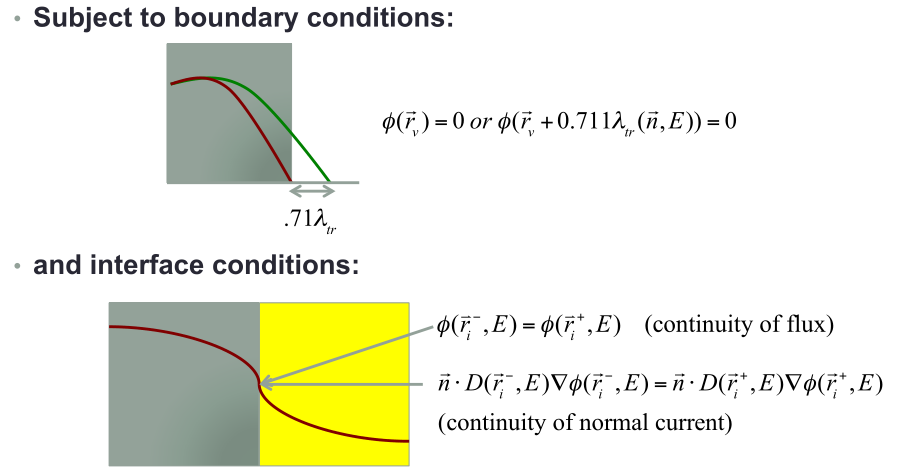
\includegraphics[width=4in]{images/dfs/boundary-interface.png}
  \caption{Boundary Conditions and Interface Conditions} \label{boundary-interface}
\end{figure}




\end{document}
